\documentclass[a4paper,12pt]{report}

\usepackage{cmap}
\usepackage[T2A]{fontenc}
\usepackage[utf8]{inputenc}
\usepackage[english,russian]{babel}
\usepackage{listings}
\usepackage{amsmath}
\usepackage{float}
\usepackage{csquotes}
\usepackage{mathtools}
\usepackage{hyphenat}
\usepackage{amsfonts}

\usepackage{xcolor}
\usepackage{hyperref}

\usepackage{graphicx}
\graphicspath{ {./images/} }

\definecolor{dkgreen}{rgb}{0,0.6,0}
\definecolor{gray}{rgb}{0.5,0.5,0.5}
\definecolor{mauve}{rgb}{0.58,0,0.82}

\lstset{
    language=Python,                 % выбор языка для подсветки (здесь это С)
    basicstyle=\small\sffamily, % размер и начертание шрифта для подсветки кода
    numbers=left,               % где поставить нумерацию строк (слева\справа)
    numberstyle=\tiny,           % размер шрифта для номеров строк
    stepnumber=1,                   % размер шага между двумя номерами строк
    numbersep=5pt,                % как далеко отстоят номера строк от подсвечиваемого кода
    aboveskip=3mm,
    belowskip=3mm,
    showstringspaces=false,
    columns=flexible,
    captionpos=b, 
    basicstyle={\small\ttfamily},
    numbers=left,
    numberstyle=\tiny\color{gray},
    keywordstyle=\color{blue},
    commentstyle=\color{mauve},
    stringstyle=\color{dkgreen},
    breaklines=true,
    breakatwhitespace=true,
    tabsize=3
}

\title{Лабораторная работа №5\\Автокорреляция}
\author{Кобыжев Александр}
\date{\today}

\begin{document}

\maketitle
\tableofcontents
\listoffigures
\lstlistoflistings

\maketitle

\chapter{Упражнение 5.1}

Позаимствуем функции из блокнота \texttt{chap05.ipynb} для выполнения данного пункта лабораторной работы.

\begin{lstlisting}[caption=Функция serial\_corr]
def serial_corr(wave, lag=1):
    N = len(wave)
    y1 = wave.ys[lag:]
    y2 = wave.ys[:N-lag]
    corr = np.corrcoef(y1, y2, ddof=0)[0, 1]
    return corr
\end{lstlisting}

\begin{lstlisting}[caption=Функция \texttt{autocorr}]
def autocorr(wave):
    lags = range(len(wave.ys)//2)
    corrs = [serial_corr(wave, lag) for lag in lags]
    return lags, corrs
\end{lstlisting}

Загрузим вокальный чирп.

\begin{lstlisting}[caption=Вокальный чирп]
wave = thinkdsp.read_wave('28042__bcjordan__voicedownbew.wav')
wave.normalize()
wave.make_audio()
\end{lstlisting}

Возьмём короткий сегмент сигнала через 0.5 секунды после начала и длительностью 0.01 секунды:

\begin{lstlisting}[caption=Первый сегмент]
segment = wave.segment(start=0.5, duration=0.01)
\end{lstlisting}

Применим автокорреляционную функцию, чтобы оценить высоту тона:

\begin{lstlisting}[caption=Оценка высоты тона]
lags, corrs = autocorr(segment)
thinkplot.plot(lags, corrs)
thinkplot.config(xlabel='Lag (index)', ylabel='Correlation', ylim=[-1, 1])
\end{lstlisting}

\begin{figure}[H]
        \centering
        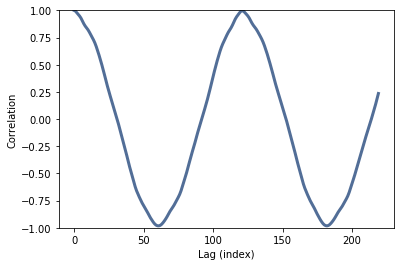
\includegraphics[width=0.75\textwidth]{lab5_fig1_1.png}
        \caption{Высота тона}
        \label{fig:lab5_fig1_1}
\end{figure}

Пик находится между 100 и 150. Используем \texttt{argmax}, чтобы уточнить значение \texttt{lag} для этого пика:

\begin{lstlisting}[caption=Нахождение \texttt{lag}]
low, high = 100, 150
lag = np.array(corrs[low:high]).argmax() + low
lag
\end{lstlisting}

Находим соответствующую частоту для \texttt{lag} = 121:

\begin{lstlisting}[caption=Нахождение частоты]
period = lag / segment.framerate
frequency = 1 / period
frequency
\end{lstlisting}

Частота равняется \texttt{364.4628099173554}.

Теперь рассмотрим сегмент сигнала через 1 секунду и проделаем аналогичные действия.

\begin{lstlisting}[caption=Второй сегмент]
segment = wave.segment(start=1.0, duration=0.01)
\end{lstlisting}

Применим автокорреляционную функцию, чтобы оценить высоту тона:

\begin{lstlisting}[caption=Оценка высоты тона]
lags, corrs = autocorr(segment)
thinkplot.plot(lags, corrs)
thinkplot.config(xlabel='Lag (index)', ylabel='Correlation', ylim=[-1, 1])
\end{lstlisting}

\begin{figure}[H]
        \centering
        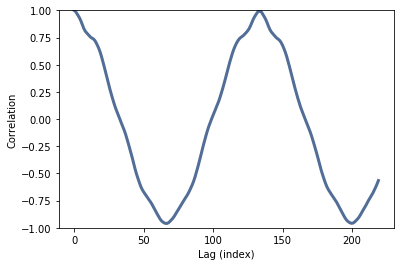
\includegraphics[width=0.75\textwidth]{lab5_fig1_2.png}
        \caption{Высота тона}
        \label{fig:lab5_fig1_2}
\end{figure}

Пик снова находится между 100 и 150. Используем \texttt{argmax}, чтобы уточнить значение \texttt{lag} для этого пика:

\begin{lstlisting}[caption=Нахождение \texttt{lag}]
low, high = 100, 150
lag = np.array(corrs[low:high]).argmax() + low
lag
\end{lstlisting}

Находим соответствующую частоту для \texttt{lag} = 134:

\begin{lstlisting}[caption=Нахождение частоты]
period = lag / segment.framerate
frequency = 1 / period
frequency
\end{lstlisting}

Частота равняется \texttt{329.1044776119403}. Отсюда можно сделать вывод, что основная частота ожидаемо уменьшается при увеличении времени начала сегмента.

\chapter{Упражнение 5.2}

Загрузим тот же вокальный чирп.

\begin{lstlisting}[caption=Загрузка звука]
wave = thinkdsp.read_wave('28042__bcjordan__voicedownbew.wav')
wave.normalize()
wave.make_audio()
\end{lstlisting}

Воспользуемся примером кода из \texttt{chap05.ipynb}. Вот его спектрограмма:

\begin{lstlisting}[caption=Спектрограмма звука]
wave.make_spectrogram(2048).plot(high=4200)
thinkplot.config(xlabel='Time (s)', 
                     ylabel='Frequency (Hz)',
                     xlim=[0, 1.4],
                     ylim=[0, 4200])
\end{lstlisting}

\begin{figure}[H]
        \centering
        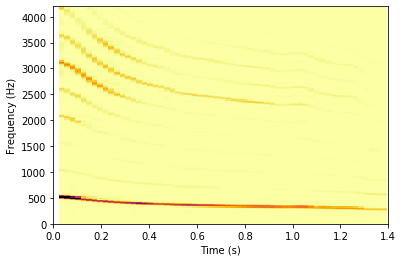
\includegraphics[width=0.75\textwidth]{lab5_fig2_1.png}
        \caption{Сегменты звуков}
        \label{fig:lab5_fig2_1}
\end{figure}

Инкапсулируем предлагаемый код в функцию. Найти первый самый высокий пик в автокорреляционной функции сложно. Поэтому мы просто укажем диапазон \texttt{lag} для поиска.

\begin{lstlisting}[caption=Инкапсуляция функции]
from autocorr import autocorr
def estimate_fundamental(segment, low=70, high=150):
    lags, corrs = autocorr(segment)
    lag = np.array(corrs[low:high]).argmax() + low
    period = lag / segment.framerate
    frequency = 1 / period
    return frequency
\end{lstlisting}

Рассмотрим пример работы функции:

\begin{lstlisting}[caption=Пример работы функции]
duration = 0.01
segment = wave.segment(start=0.2, duration=duration)
freq = estimate_fundamental(segment)
freq
\end{lstlisting}

Результатом работы получилась частота \texttt{436.63366336633663}.

Используем написанную функцию для отслеживания высоты тона записанного звука. \texttt{ts} - средние точки каждого сегмента.

\begin{lstlisting}[caption=Отслеживание высоты тона]
step = 0.05
starts = np.arange(0.0, 1.4, step)

ts = []
freqs = []

for start in starts:
    ts.append(start + step/2)
    segment = wave.segment(start=start, duration=duration)
    freq = estimate_fundamental(segment)
    freqs.append(freq)
\end{lstlisting}

Рассмотрим кривую отслеживания высоты тона, наложенную на спектрограмму:

\begin{lstlisting}[caption=Кривая отслеживания высоты тона на спектрограмме]
wave.make_spectrogram(2048).plot(high=900)
thinkplot.plot(ts, freqs, color='green')
thinkplot.config(xlabel='Time (s)', 
                     ylabel='Frequency (Hz)',
                     xlim=[0, 1.4],
                     ylim=[0, 900])
\end{lstlisting}

\begin{figure}[H]
        \centering
        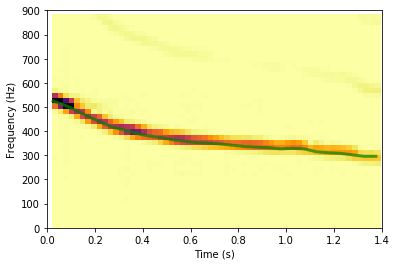
\includegraphics[width=0.75\textwidth]{lab5_fig2_2.png}
        \caption{Кривая отслеживания высоты тона на спектрограмме}
        \label{fig:lab5_fig2_2}
\end{figure}

Наложив оценки высоты тона на спектрограмму записи, можно видеть, что функция полностью справляется со своей задачей.

\chapter{Упражнение 5.3}

Воспользуемся данными о ежедневной цене \texttt{BitCoin} в течение года из прошлой лабораторной работы.

\begin{lstlisting}[caption=Таблица данных]
data = pd.read_csv('BTC_USD_2020-04-08_2021-04-07-CoinDesk.csv')
data
\end{lstlisting}

\begin{figure}[H]
        \centering
        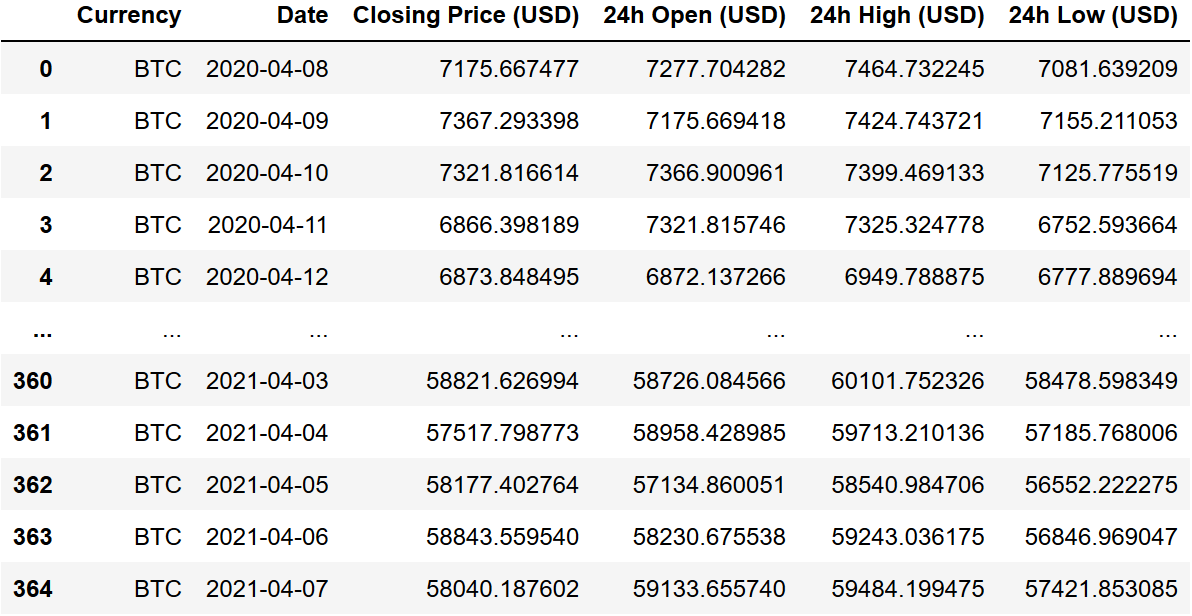
\includegraphics[width=0.75\textwidth]{lab5_fig3_1.png}
        \caption{Таблица данных}
        \label{fig:lab5_fig3_1}
\end{figure}

Визуализируем скачанные данные.

\begin{lstlisting}[caption=Визуализация данных]
wave = thinkdsp.Wave(data['Closing Price (USD)'], data.index, framerate=1)
wave.plot()
thinkplot.config(xlabel='Time (days)',
                 ylabel='Price of BitCoin ($)')
\end{lstlisting}

\begin{figure}[H]
        \centering
        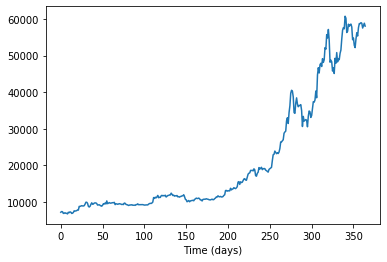
\includegraphics[width=0.75\textwidth]{lab5_fig3_2.png}
        \caption{Визуализация данных}
        \label{fig:lab5_fig3_2}
\end{figure}

Воспользуемся функцией автокорреляции, использующая статистическое определение, то есть она сдвигает среднее значение к нулю, делит на стандартное отклонение и делит сумму на N.

\begin{lstlisting}[caption=Автокорреляция при помощи \texttt{autocorr}]
from autocorr import autocorr

lags, corrs = autocorr(wave)
thinkplot.plot(lags, corrs)
thinkplot.config(xlabel='Lag',
                 ylabel='Correlation')
\end{lstlisting}

\begin{figure}[H]
        \centering
        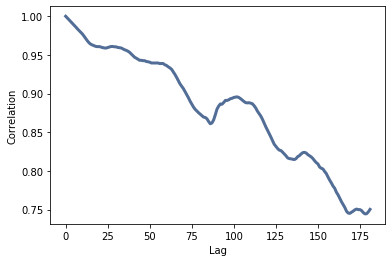
\includegraphics[width=0.75\textwidth]{lab5_fig3_3.png}
        \caption{Автокорреляция при помощи \texttt{autocorr}}
        \label{fig:lab5_fig3_3}
\end{figure}

Автокорреляционная функция падает медленно, поскольку задержка увеличивается, предполагая какой-то розовый шум.

Мы можем сравнить реализацию \texttt{autocorr} с \texttt{np.correlate}, в котором используется определение корреляции, используемое при обработке сигналов.

\begin{lstlisting}[caption=Автокорреляция при помощи \texttt{np.correlate}]
N = len(wave)
corrs2 = np.correlate(wave.ys, wave.ys, mode='same')
lags = np.arange(-N//2, N//2)
thinkplot.plot(lags, corrs2)
thinkplot.config(xlabel='Lag',
                 ylabel='Dot product')
\end{lstlisting}

\begin{figure}[H]
        \centering
        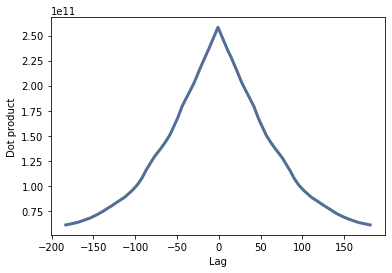
\includegraphics[width=0.75\textwidth]{lab5_fig3_4.png}
        \caption{Автокорреляция при помощи \texttt{np.correlate}}
        \label{fig:lab5_fig3_4}
\end{figure}

Результат симметричен, потому что два сигнала идентичны, и отрицательный \texttt{lag} у одного даёт такой же эффект, как и положительный \texttt{lag} у другого. Вторая половина результата соответствует положительным \texttt{lag}:

\begin{lstlisting}[caption=Вторая половина результата]
N = len(corrs2)
half = corrs2[N//2:]
thinkplot.plot(half)
thinkplot.config(xlabel='Lag',
                 ylabel='Dot product')
\end{lstlisting}

\begin{figure}[H]
        \centering
        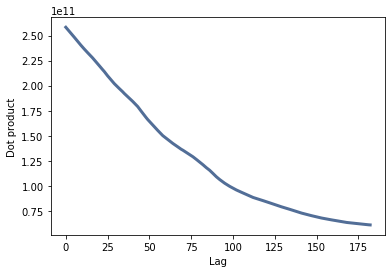
\includegraphics[width=0.75\textwidth]{lab5_fig3_5.png}
        \caption{Вторая половина результата}
        \label{fig:lab5_fig3_5}
\end{figure}

Мы можем нормализовать результаты, разделив их на длины (\texttt{lengths}):

\begin{lstlisting}[caption=Нормализованный результат]
lengths = range(N, N//2, -1)
half /= lengths
half /= half[0]
thinkplot.plot(half)
thinkplot.config(xlabel='Lag',
                 ylabel='Dot product')
\end{lstlisting}

\begin{figure}[H]
        \centering
        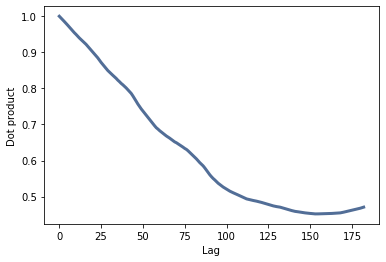
\includegraphics[width=0.75\textwidth]{lab5_fig3_6.png}
        \caption{Нормализованный результат}
        \label{fig:lab5_fig3_6}
\end{figure}

Но даже после нормализации результаты выглядят совершенно по-другому. В результате корреляции пики стираются.

\begin{lstlisting}[caption=Сравнение результатов]
thinkplot.preplot(2)
thinkplot.plot(corrs, label='autocorr')
thinkplot.plot(half, label='correlate')
thinkplot.config(xlabel='Lag', ylabel='Correlation')
\end{lstlisting}

\begin{figure}[H]
        \centering
        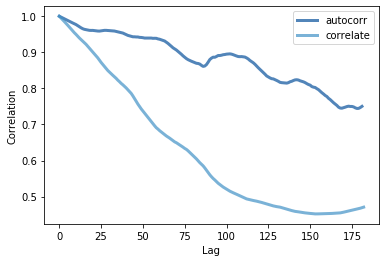
\includegraphics[width=0.75\textwidth]{lab5_fig3_7.png}
        \caption{Сравнение результатов}
        \label{fig:lab5_fig3_7}
\end{figure}

Скорее всего причина различия результатов в том, что данные выглядят очень по-разному в разных частях диапазона, в частности, дисперсия сильно меняется с течением времени.

Для этого набора данных, вероятно, более уместно статистическое определение автокорреляционной функции.

\chapter{Упражнение 5.4}

Для выполнения данного задания я нашёл другой звук саксофона, который можно прослушать по  \href{https://freesound.org/people/felix.blume/sounds/414062/}{\texttt{ссылке}}.

\begin{lstlisting}[caption=Загрузка звука]
wave = thinkdsp.read_wave('77685__juskiddink__anna-britta-sax.wav')
wave.normalize()
wave.make_audio()
\end{lstlisting}

Рассмотрим спектрограмму, которая показывает гармоническую структуру во времени.

\begin{lstlisting}[caption=Спектрограмма звука]
gram = wave.make_spectrogram(seg_length=1024)
gram.plot(high=3000)
thinkplot.config(xlabel='Time (s)', ylabel='Frequency (Hz)')
\end{lstlisting}

\begin{figure}[H]
        \centering
        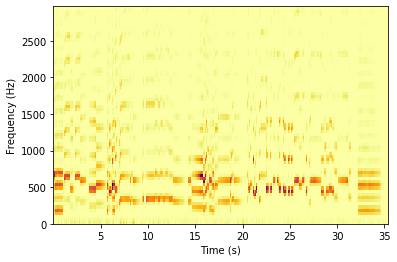
\includegraphics[width=0.75\textwidth]{lab5_fig4_1.png}
        \caption{Спектрограмма звука}
        \label{fig:lab5_fig4_1}
\end{figure}

Чтобы увидеть гармоники более четко, я возьму сегмент от 3 секунд продолжительностью 0.5 секунды и вычислю его спектр.

\begin{lstlisting}[caption=Создание сегмента звука]
start = 3.0
duration = 0.5
segment = wave.segment(start=start, duration=duration)
segment.make_audio()
\end{lstlisting}

\begin{lstlisting}[caption=Спектр звука]
spectrum = segment.make_spectrum()
spectrum.plot(high=3000)
thinkplot.config(xlabel='Frequency (Hz)', ylabel='Amplitude')
\end{lstlisting}

\begin{figure}[H]
        \centering
        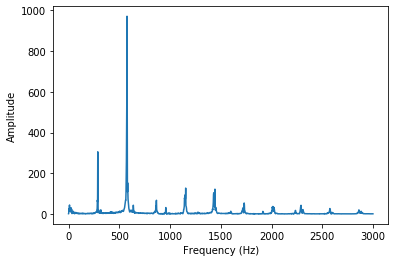
\includegraphics[width=0.75\textwidth]{lab5_fig4_2.png}
        \caption{Спектр звука}
        \label{fig:lab5_fig4_2}
\end{figure}

Пики в спектре находятся на частотах 288, 576 и 1154 Гц.

Высота звука, которую мы воспринимаем, является основной, на частоте 288 Гц, хотя она и не является доминирующей частотой.

Для сравнения, рассмотрим треугольную волну на частоте 288 Гц.

\begin{lstlisting}[caption=Треугольная волна]
thinkdsp.TriangleSignal(freq=288).make_wave(duration=0.5).make_audio()
\end{lstlisting}

\begin{lstlisting}[caption=Сегмент звука]
segment.make_audio()
\end{lstlisting}

У них одинаковая воспринимаемая высота тона. Чтобы понять, почему мы воспринимаем основную частоту, даже если она не является доминирующей, полезно взглянуть на функцию автокорреляции (АКФ). Написанная функция вычисляет АКФ, выбирает вторую половину (которая соответствует положительным \texttt{lag}) и нормализует результаты:

\begin{lstlisting}[caption=Функция \texttt{autocorr}]
def autocorr(segment):
    corrs = np.correlate(segment.ys, segment.ys, mode='same')
    N = len(corrs)
    lengths = range(N, N//2, -1)

    half = corrs[N//2:].copy()
    half /= lengths
    half /= half[0]
    return half
\end{lstlisting}

\begin{lstlisting}[caption=Визуализация АКФ]
corrs = autocorr(segment)
thinkplot.plot(corrs[:200])
thinkplot.config(xlabel='Lag', ylabel='Correlation', ylim=[-1.05, 1.05])
\end{lstlisting}

\begin{figure}[H]
        \centering
        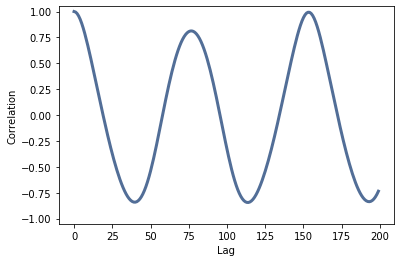
\includegraphics[width=0.75\textwidth]{lab5_fig4_3.png}
        \caption{Визуализация АКФ}
        \label{fig:lab5_fig4_3}
\end{figure}

Первый крупный пик находится вблизи \texttt{lag} = 75.

Следующая написанная функция находит самую высокую корреляцию в заданном диапазоне лагов и возвращает соответствующую частоту.

\begin{lstlisting}[caption=Функция find\_frequency]
def find_frequency(corrs, low, high):
    lag = np.array(corrs[low:high]).argmax() + low
    print(lag)
    period = lag / segment.framerate
    frequency = 1 / period
    return frequency
    
find_frequency(corrs, 65, 90)
\end{lstlisting}

Наибольший пик приходится на \texttt{lag} 77, что соответствует частоте 572.(72) Гц.

По крайней мере, в этом примере воспринимаемый нами шаг соответствует самому высокому пику автокорреляционной функции (АКФ), а не самому высокому компоненту спектра.

Удивительно, но воспринимаемый шаг не меняется, если мы полностью удаляем фундаментальный. Вот как выглядит спектр, если мы используем фильтр высоких частот, чтобы убрать фундаментальный.

\begin{lstlisting}[caption=Отфильтрованный спектр]
spectrum2 = segment.make_spectrum()
spectrum2.high_pass(600)
spectrum2.plot(high=3000)
thinkplot.config(xlabel='Frequency (Hz)', ylabel='Amplitude')
\end{lstlisting}

\begin{figure}[H]
        \centering
        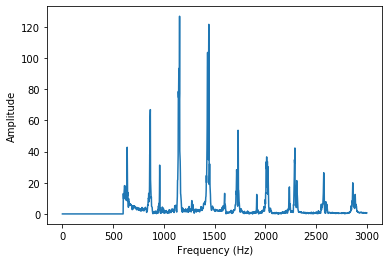
\includegraphics[width=0.75\textwidth]{lab5_fig4_4.png}
        \caption{Отфильтрованный спектр}
        \label{fig:lab5_fig4_4}
\end{figure}

Прослушаем полученный сегмент.

\begin{lstlisting}[caption=Прослушивание сегмента]
segment2 = spectrum2.make_wave()
segment2.make_audio()
\end{lstlisting}

Воспринимаемый шаг всё ещё составляет 288 Гц, хотя на этой частоте нет мощности. Это явление называется "недостающим фундаментальным".

Чтобы понять, почему мы слышим частоту, которой нет в сигнале, полезно взглянуть на функцию автокорреляции.

\begin{lstlisting}[caption=Визуализация АКФ]
corrs = autocorr(segment2)
thinkplot.plot(corrs[:200])
thinkplot.config(xlabel='Lag', ylabel='Correlation', ylim=[-1.05, 1.05])
\end{lstlisting}

\begin{figure}[H]
        \centering
        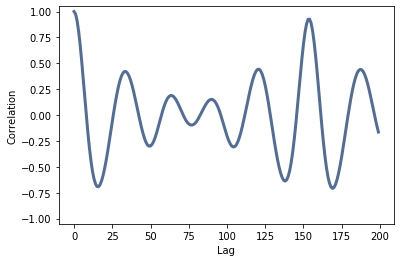
\includegraphics[width=0.75\textwidth]{lab5_fig4_5.png}
        \caption{Визуализация АКФ}
        \label{fig:lab5_fig4_5}
\end{figure}

Пятый пик, который соответствует 288 Гц, по-прежнему самый высокий. Остальные пики не являются гармониками.

Так почему же мы не воспринимаем ни одну из этих частот вместо 288 Гц? Причина в том, что высшие компоненты, присутствующие в сигнале, являются гармониками 288 Гц, а не гармониками 364,490,689 или 1336 Гц.

Наше ухо интерпретирует высокие гармоники как свидетельство того, что "правильный" фундаментал находится на частоте 288 Гц.

Если мы избавимся от высоких гармоник, эффект исчезнет. Рассмотрим спектр с удалёнными гармониками выше 1200 Гц.

\begin{lstlisting}[caption=Спектр с удалёнными гармониками]
spectrum4 = segment.make_spectrum()
spectrum4.high_pass(1000)
spectrum4.low_pass(1200)
spectrum4.plot(high=3000)
thinkplot.config(xlabel='Frequency (Hz)', ylabel='Amplitude')
\end{lstlisting}

\begin{figure}[H]
        \centering
        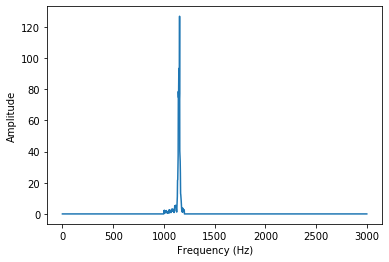
\includegraphics[width=0.75\textwidth]{lab5_fig4_6.png}
        \caption{Спектр с удалёнными гармониками}
        \label{fig:lab5_fig4_6}
\end{figure}

Теперь воспринимаемая частота составляет 1200 Гц.

\begin{lstlisting}[caption=Прослушивание нового звука]
segment4 = spectrum4.make_wave()
segment4.make_audio()
\end{lstlisting}

\begin{lstlisting}[caption=Треугольный сигнал на 1200 Гц]
thinkdsp.TriangleSignal(freq=1200).make_wave(duration=0.5).make_audio()
\end{lstlisting}

\begin{lstlisting}[caption=Визуализация АКФ]
corrs = autocorr(segment4)
thinkplot.plot(corrs[:200])
thinkplot.config(xlabel='Lag', ylabel='Correlation', ylim=[-1.05, 1.05])
\end{lstlisting}

\begin{figure}[H]
        \centering
        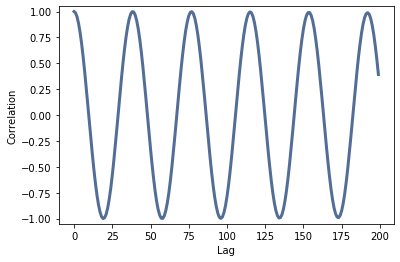
\includegraphics[width=0.75\textwidth]{lab5_fig4_7.png}
        \caption{Визуализация АКФ}
        \label{fig:lab5_fig4_7}
\end{figure}

\begin{lstlisting}[caption=Поиск пика]
find_frequency(corrs, 25, 50)
\end{lstlisting}

А если мы посмотрим на автокорреляционную функцию, то найдем самый высокий пик при \texttt{lag} = 38, что соответствует 1160 Гц.

Таким образом, эти эксперименты показывают, что восприятие высоты тона не полностью основано на спектральном анализе, но также информируется чем-то вроде автокорреляции.

\chapter{Выводы}

Во время выполнения лабораторной работы получены навыки работы с корреляцией, последовательной корреляцей, автокорреляцей. Также рассмотрена автокорреляционная функция (АКФ).

\end{document}